%
% Capítulo 4
%
\chapter{Architecture} \label{cap:architecture}

This chapter provides an overview of the system’s components and their interactions.
It outlines the capabilities of the project and presents the architecture, entities, and
implementation blueprint that have been designed and developed.

\section{Overview}

Figure ~\ref{fig:architecture} presents a diagram illustrating the main components of the system and their interactions. The system consists of a backend application (server-side) and a frontend application (client-side).
The backend architecture consists of routes, services, and repositories. The routes handle incoming HTTP requests and call the appropriate service. The services manage data manipulation, validation, and interactions with external APIs or databases. Finally, the processed data is sent to the repositories, which store it in the database.

\begin{figure}[H]
	\begin{center}
		\resizebox{160mm}{!}{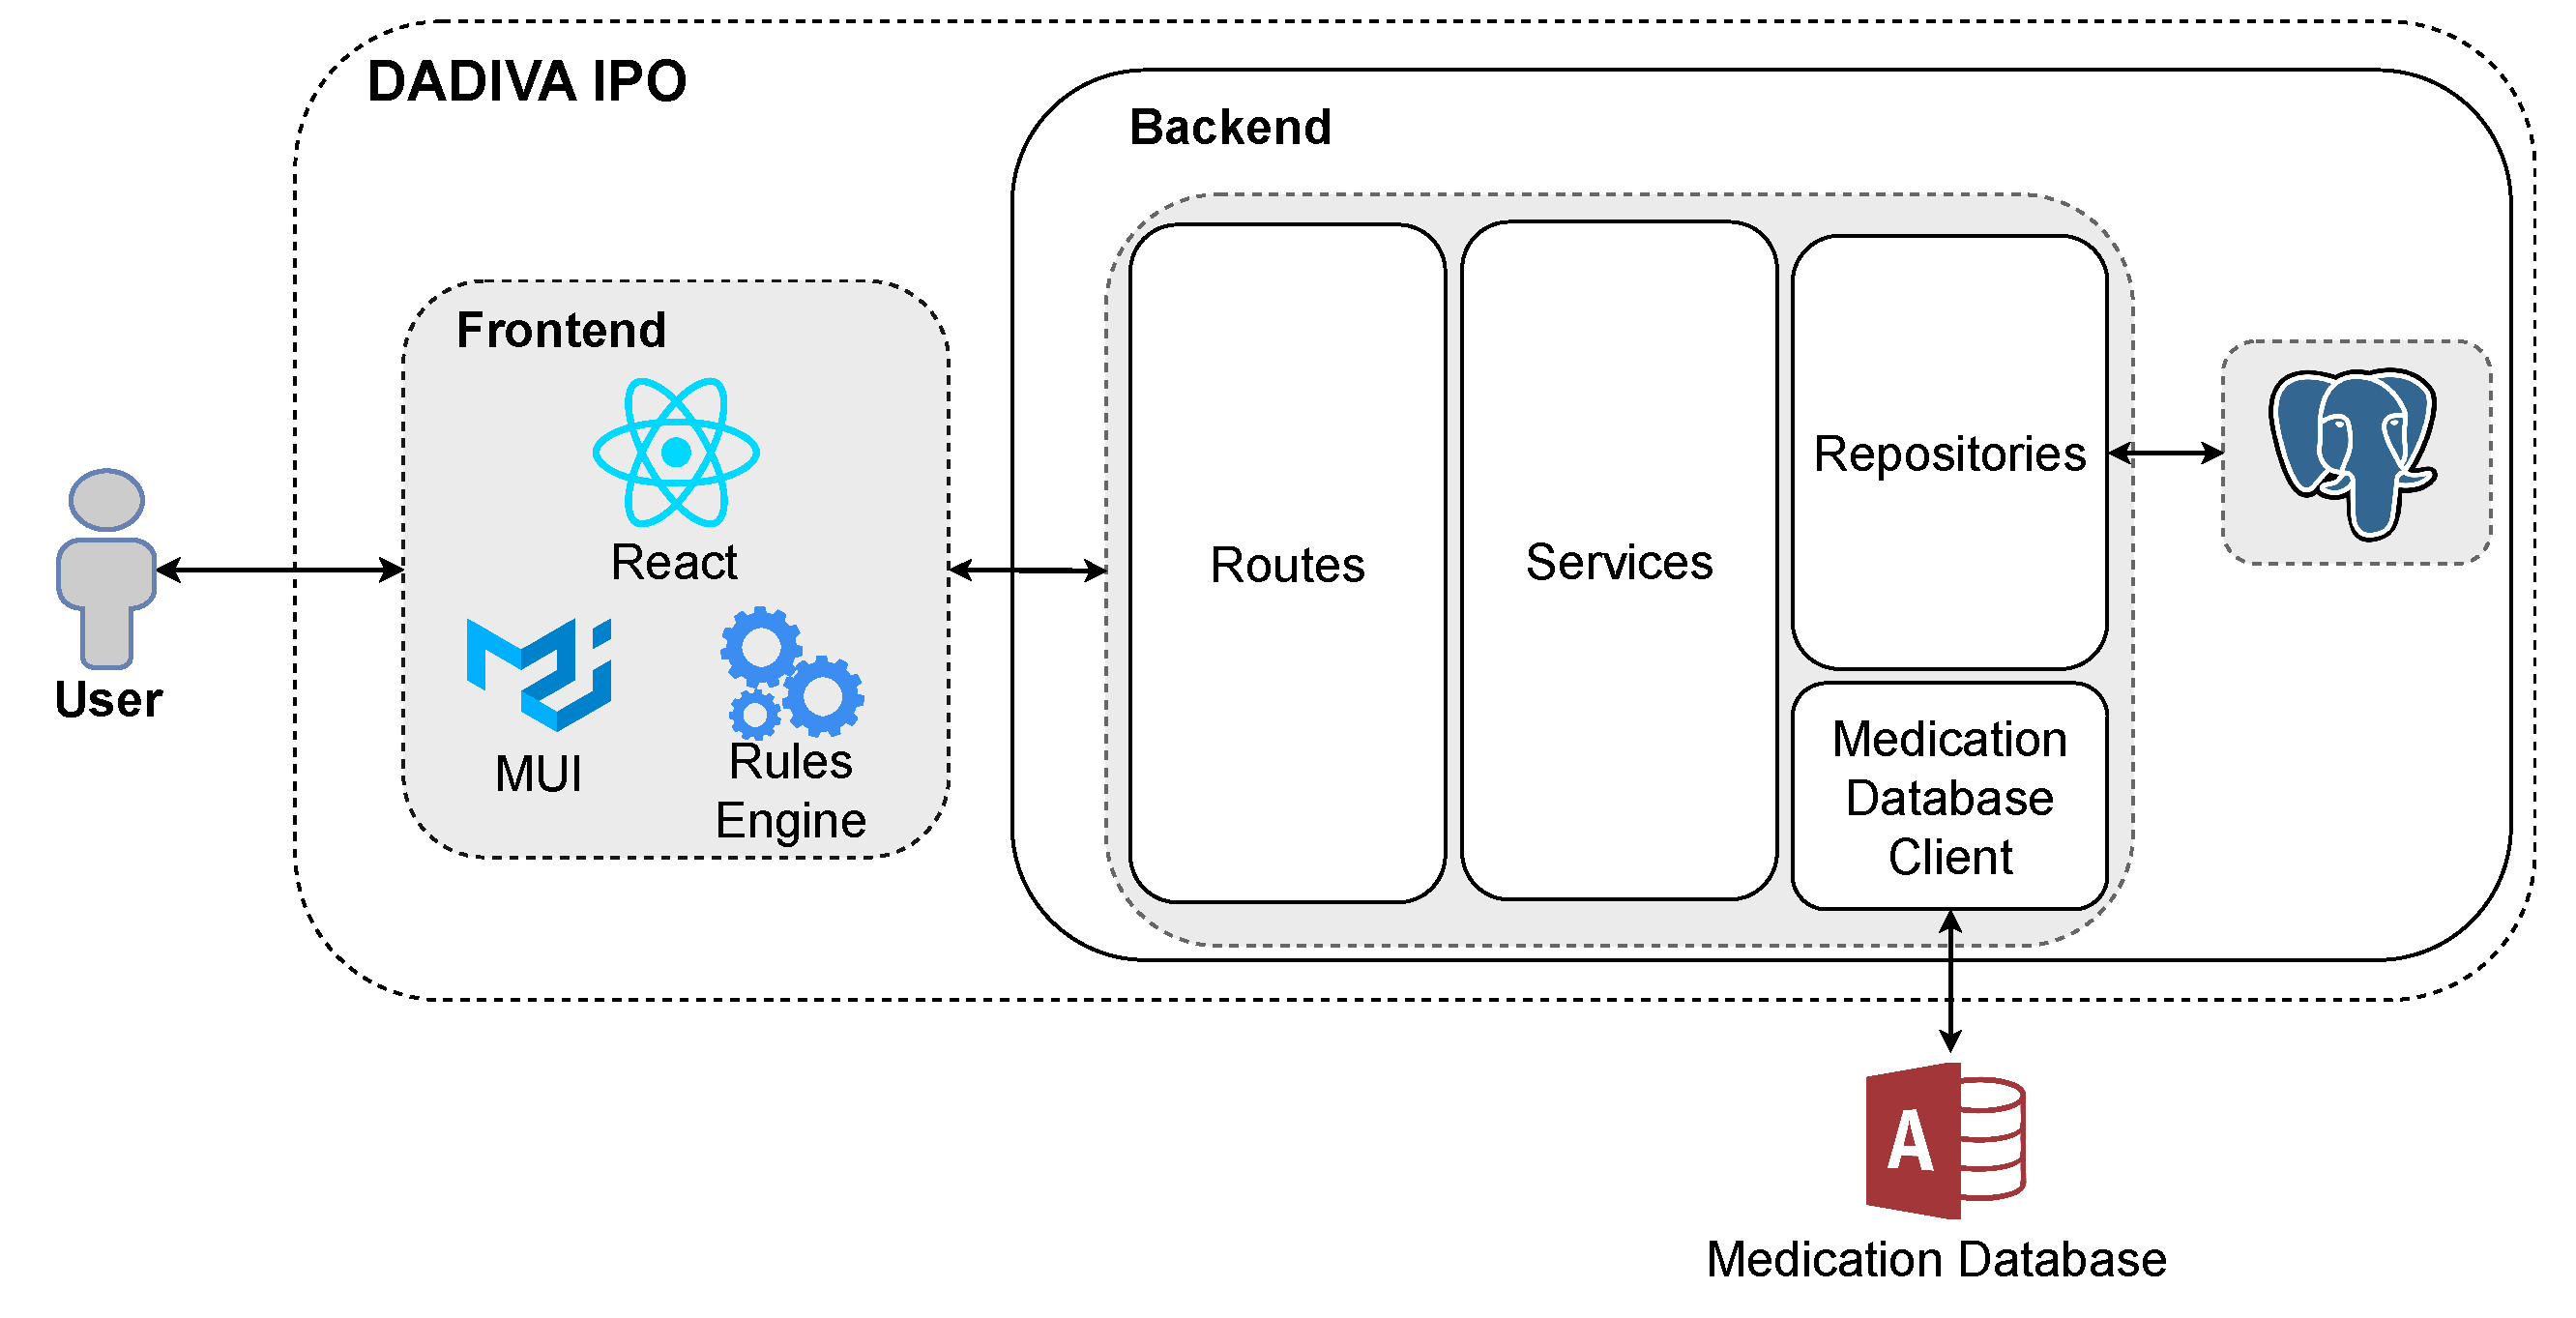
\includegraphics{./figures/Architecture.pdf}}
	\end{center}
	\caption{Application Architecture, gray squares represent containerized components of the solution.}\label{fig:architecture}
\end{figure}

\section{Backend Application}

The backend application can be abstracted into 3 layers:
\begin{itemize}
	\item routes: responsible for receiving the http request and calling the correct service;
	\item services: contains the services that manage the business logic of the application;
	\item repositories: contains the repository layer of the application, uses the ElasticSearchClient;
\end{itemize}


%The backend handles HTTP requests directed to specific endpoints. The route associated with each endpoint converts the request body into an appropriate model, if necessary, and then calls the corresponding service, passing along the model. The service validates the model, converts it into a domain object, and calls the relevant repository. Using an ElasticClient, the repository stores the object in the ElasticSearch database. The appropriate response is then propagated back up, as illustrated in Figure ~\ref{fig:backendLayers}.
%
%\begin{figure}[H]
%	\begin{center}
%		\resizebox{100mm}{!}{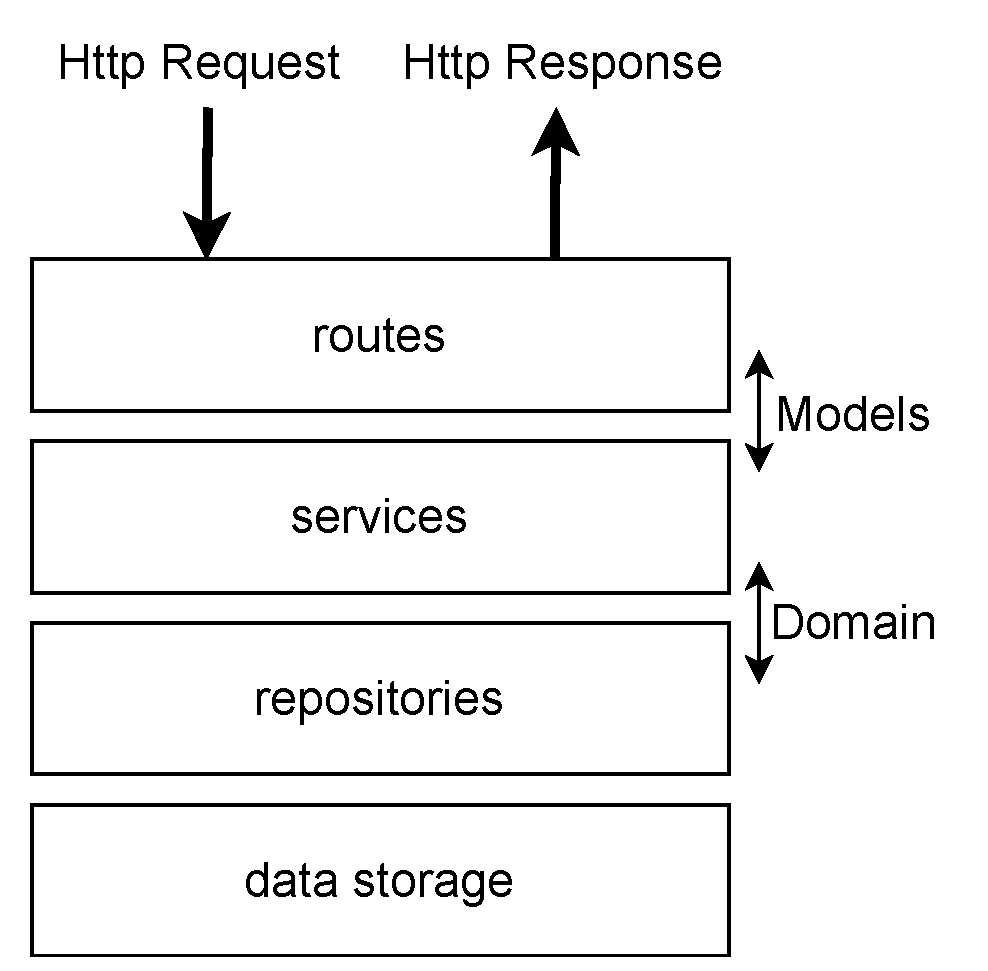
\includegraphics{./figures/backendLayers.pdf}}
%	\end{center}
%	\caption{Backend layers.}\label{fig:backendLayers}
%\end{figure}

The service layer is composed by the following elements:

\begin{itemize}
	\item form: responsible for form management, such as, creation, requests, submission, editing and deletion;
	\item search: responsible for medication and pathology interaction information retrieval;
	\item users: responsible for user management, such as, registration, login, deletion and role management.
\end{itemize}

The repositories communicate with the database, in which the various data models are divided into specific indexes, such as:

\begin{itemize}
	\item /form: stores all the form structures;
	\item /submissions: stores all the user form responses;
	\item /inconsistencies: stores all the user form inconsistencies;
	\item /users: stores all the users.
\end{itemize}

An example of a GET request for the form resource is presented in Figure ~\ref{fig:getForm_Sequence_Diagram}

\begin{figure}[H]
	\begin{center}
		\resizebox{160mm}{!}{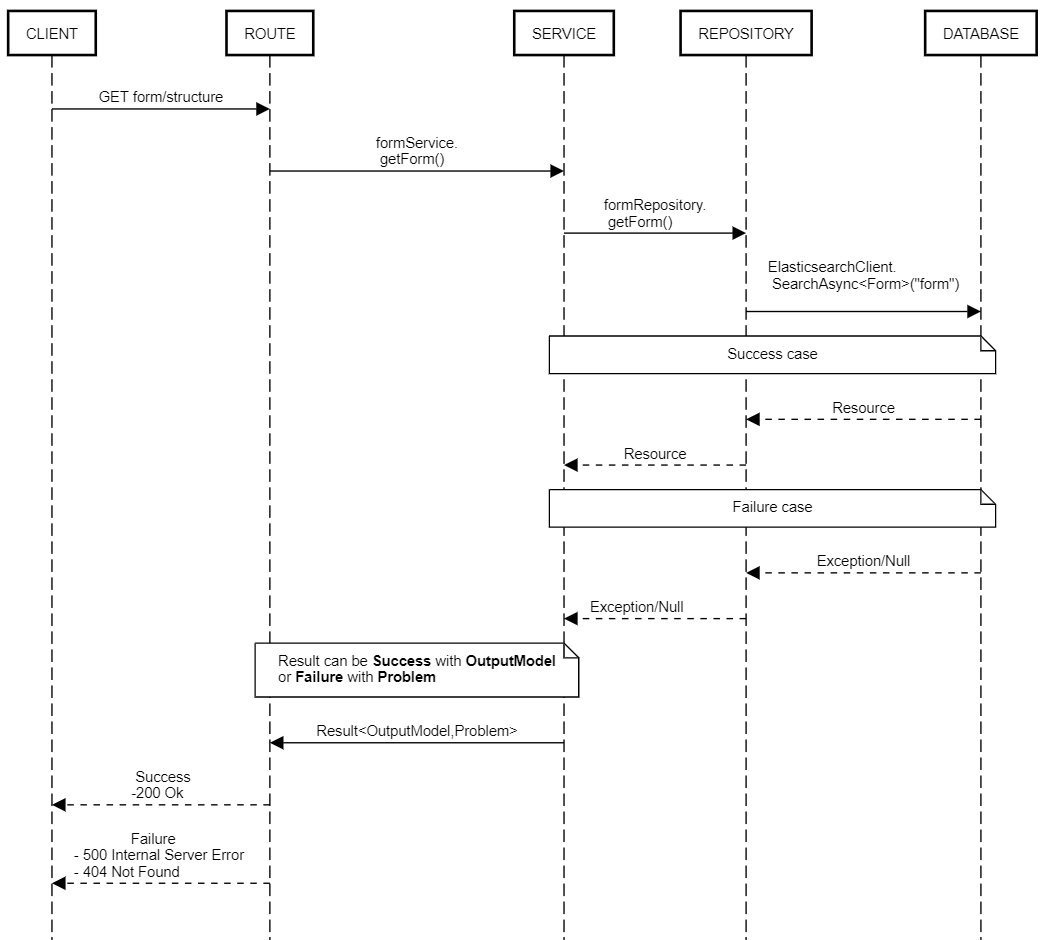
\includegraphics{./figures/getForm_Sequence_Diagram.png}}
	\end{center}
	\caption{Get Form Sequence Diagram.}\label{fig:getForm_Sequence_Diagram}
\end{figure}


\section{Form Data Model and Inconsistencies Data Model}

The first approach to solve the dynamic form challenge was to use a data structure formed by pairs of main questions and sub-questions, example presented in Figure ~\ref{fig:old_form}, where a main question can only be answered with boolean values, and one of those values triggers the display of a sub-question which has a certain type of response, such as boolean, dropdown for known multiple answers, and text, to accept user text input.

\begin{figure}[hbt!]
	\begin{center}
		\resizebox{150mm}{!}{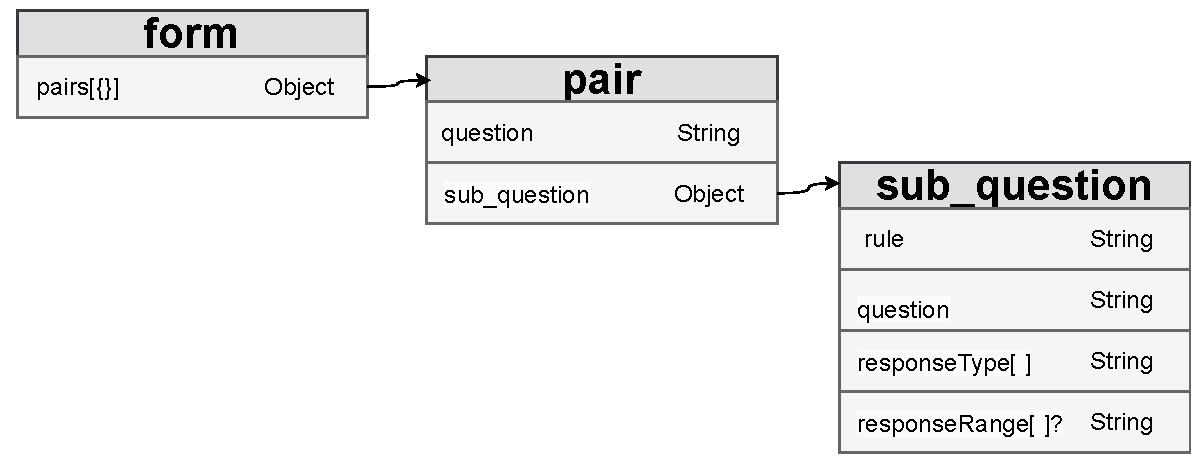
\includegraphics{./figures/oldForm.pdf}}
	\end{center}
	\caption{First Form Data Structure.}\label{fig:old_form}
\end{figure}

This approach has several drawbacks. Firstly, it prevents the suppression of further questions, which contradicts the goal of creating a flexible and adaptable solution. Additionally, it conflates questions and rules within sub-questions, leading to a lack of clarity and potential confusion in implementation.

Upon further discussion we settled on using a more complex data structure , exemplified in Figure ~\ref{fig:new_form}, composed by a list of questions and a list of rules.

Each question has an id, the text that composes it, the type of response (boolean, text and dropdown) and can have options that lists all the possibles values for a multiple(dropdown) response.

Each rule has conditions, which can be "any","all" or "not", so that, when any, all or none of the conditions are met an event is triggered.
Each condition type will have a fact, an operator and a value. In essence, when a question, which is identified by the fact field via it's id, is answered a condition can true or false depending on the logical operator used, ie equal or notEqual, and the value of the answer. If the condition is true an event is triggered, this event can be to show or hide a subsequent question, this targeted question is identified via the id, supplied in the params field.

This model, specifically the rules field, was chosen as it is part of the JSON-Rules-Engine specification, which is presented in more detail in Chapter ~\ref{cap:technologies} and is easily stored and retrieved in a ElasticSearch database.

\begin{figure}[htbp]
	\begin{center}
		{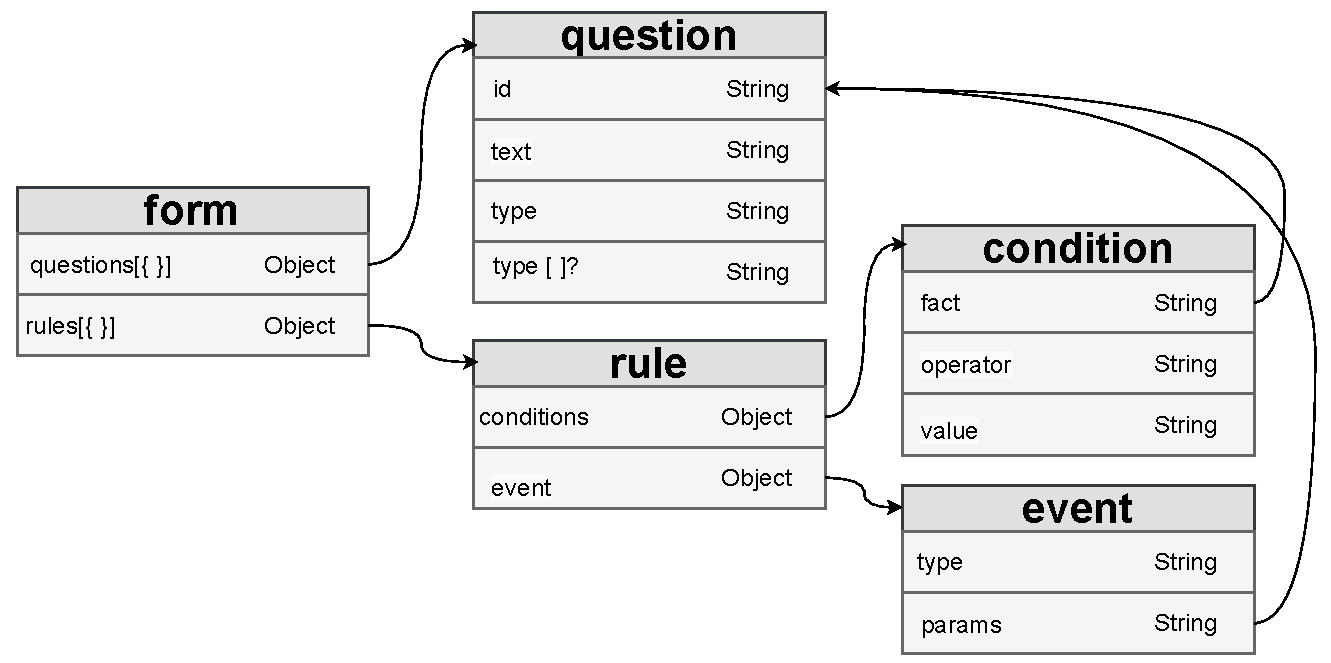
\includegraphics[width=\textwidth,height=\textheight,keepaspectratio]{./figures/newForm.pdf}}
	\end{center}
	\caption{Final Form Data Structure.}\label{fig:new_form}
\end{figure}
\FloatBarrier

The inconsistencies data model is compromised of rules, and describes answer combinations that are logical fallacies, ie a donor answering that they're healthy in one question and that they have a chronic disease in another question.

\section{Submission Data Model}

The submission data structure represents and answered form, has such it contains a list of answered questions, each answered question is composed by the question id and the answer, as referenced in Figure ~\ref{fig:submission_data_model}.

\begin{figure}[hbt!]
	\begin{center}
		\resizebox{150mm}{!}{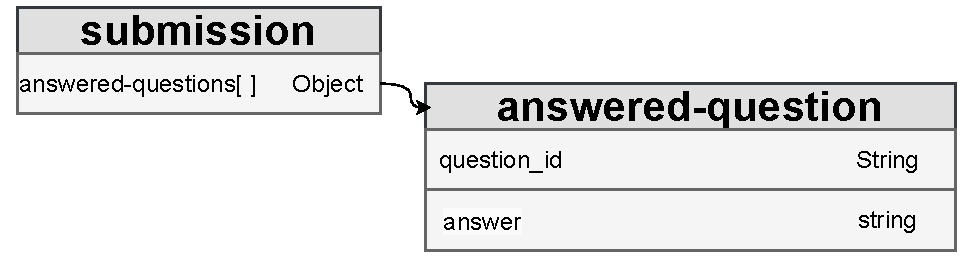
\includegraphics{./figures/Submission_Data_Model.pdf}}
	\end{center}
	\caption{Submission Data Structure.}\label{fig:submission_data_model}
\end{figure}


\section{User Data Model}

The user data structure is composed on an unique identifier, the nic, and the user hashed password, as referenced in Figure ~\ref{fig:user_data_model}.

\begin{figure}[hbt!]
	\begin{center}
		\resizebox{150mm}{!}{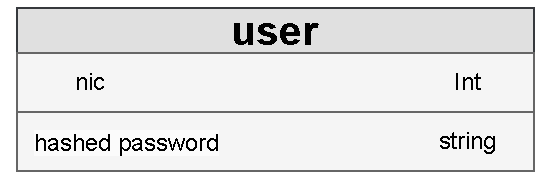
\includegraphics{./figures/User_Data_Structure.pdf}}
	\end{center}
	\caption{User Data Structure.}\label{fig:user_data_model}
\end{figure}

%%secalhar é mais adequado na descrição do problema
\section{IPO Medication Portal}
\textcolor{red}{
The IPST medication guideline are organized in a table like manner, in the following column layout:
	\begin{enumerate}
		\item Class/Group of Medication: This column categorizes medications.
		\item Active Substance/Commercial Name: This column lists either the active ingredient or the brand name of the medication.
		\item Criteria: This column specifies if a particular class or group of medications affects eligibility for blood donation, including details such as the duration of ineligibility and other relevant conditions.
	\end{enumerate}
	The terms used in the first column are, from what we can access, similar to the available pharmacotherapeutic classifications. A reliable source of a drug's pharmacotherapeutic classification is a portal provided by Infarmed to it's partner organizations, such as Lisbon's IPO.
	As such, upon a donor's form submission, assuming they where taking some medication, our application would perform requests to said portal, get the appropriate pharmacotherapeutic classification and, by cross-checking the classification with the term used in the first column of the guidelines, return the relevant information.
	However the terms used in the guidelines don't always reflect the available classifications, and, as such, the platform will employ a dictionary that associates the terms used in the guidelines to pharmacotherapeutic classifications. This dictionary will be updatable by the platform's administrators.
	The fact that the IPST guidelines aren't available in a machine readable format persists.
}

\section{Frontend Application}\label{architecture_frontend}

The frontend application is a web-based interface designed to facilitate seamless interaction between users and the backend system. It features a user-friendly and intuitive interface, catering to different types of users with specific functionalities:

\begin{itemize}
	\item Donor Users: Can fill out the current donation form;
	\item Doctor Users: Can search for pathology and medication interactions with blood donation and request form answers for specific users;
	\item Administrator Users: Can customize the current form, update pathology and medication interaction information, and manage users.
\end{itemize}

The application is organized into multiple pages and components, each serving distinct purposes. It includes a service layer responsible for communicating with the backend application through the REST API.

During planning some mockups where created of the final result for some pages, the login page is presented in Figure ~\ref{fig:login}, the form pages are presented in Figures ~\ref{fig:form},~\ref{fig:form_no} and ~\ref{fig:form_yes}, the backoffice page is presented in Figure ~\ref{fig:backoffice}.

\begin{figure}[H]
	\begin{center}
		\resizebox{160mm}{!}{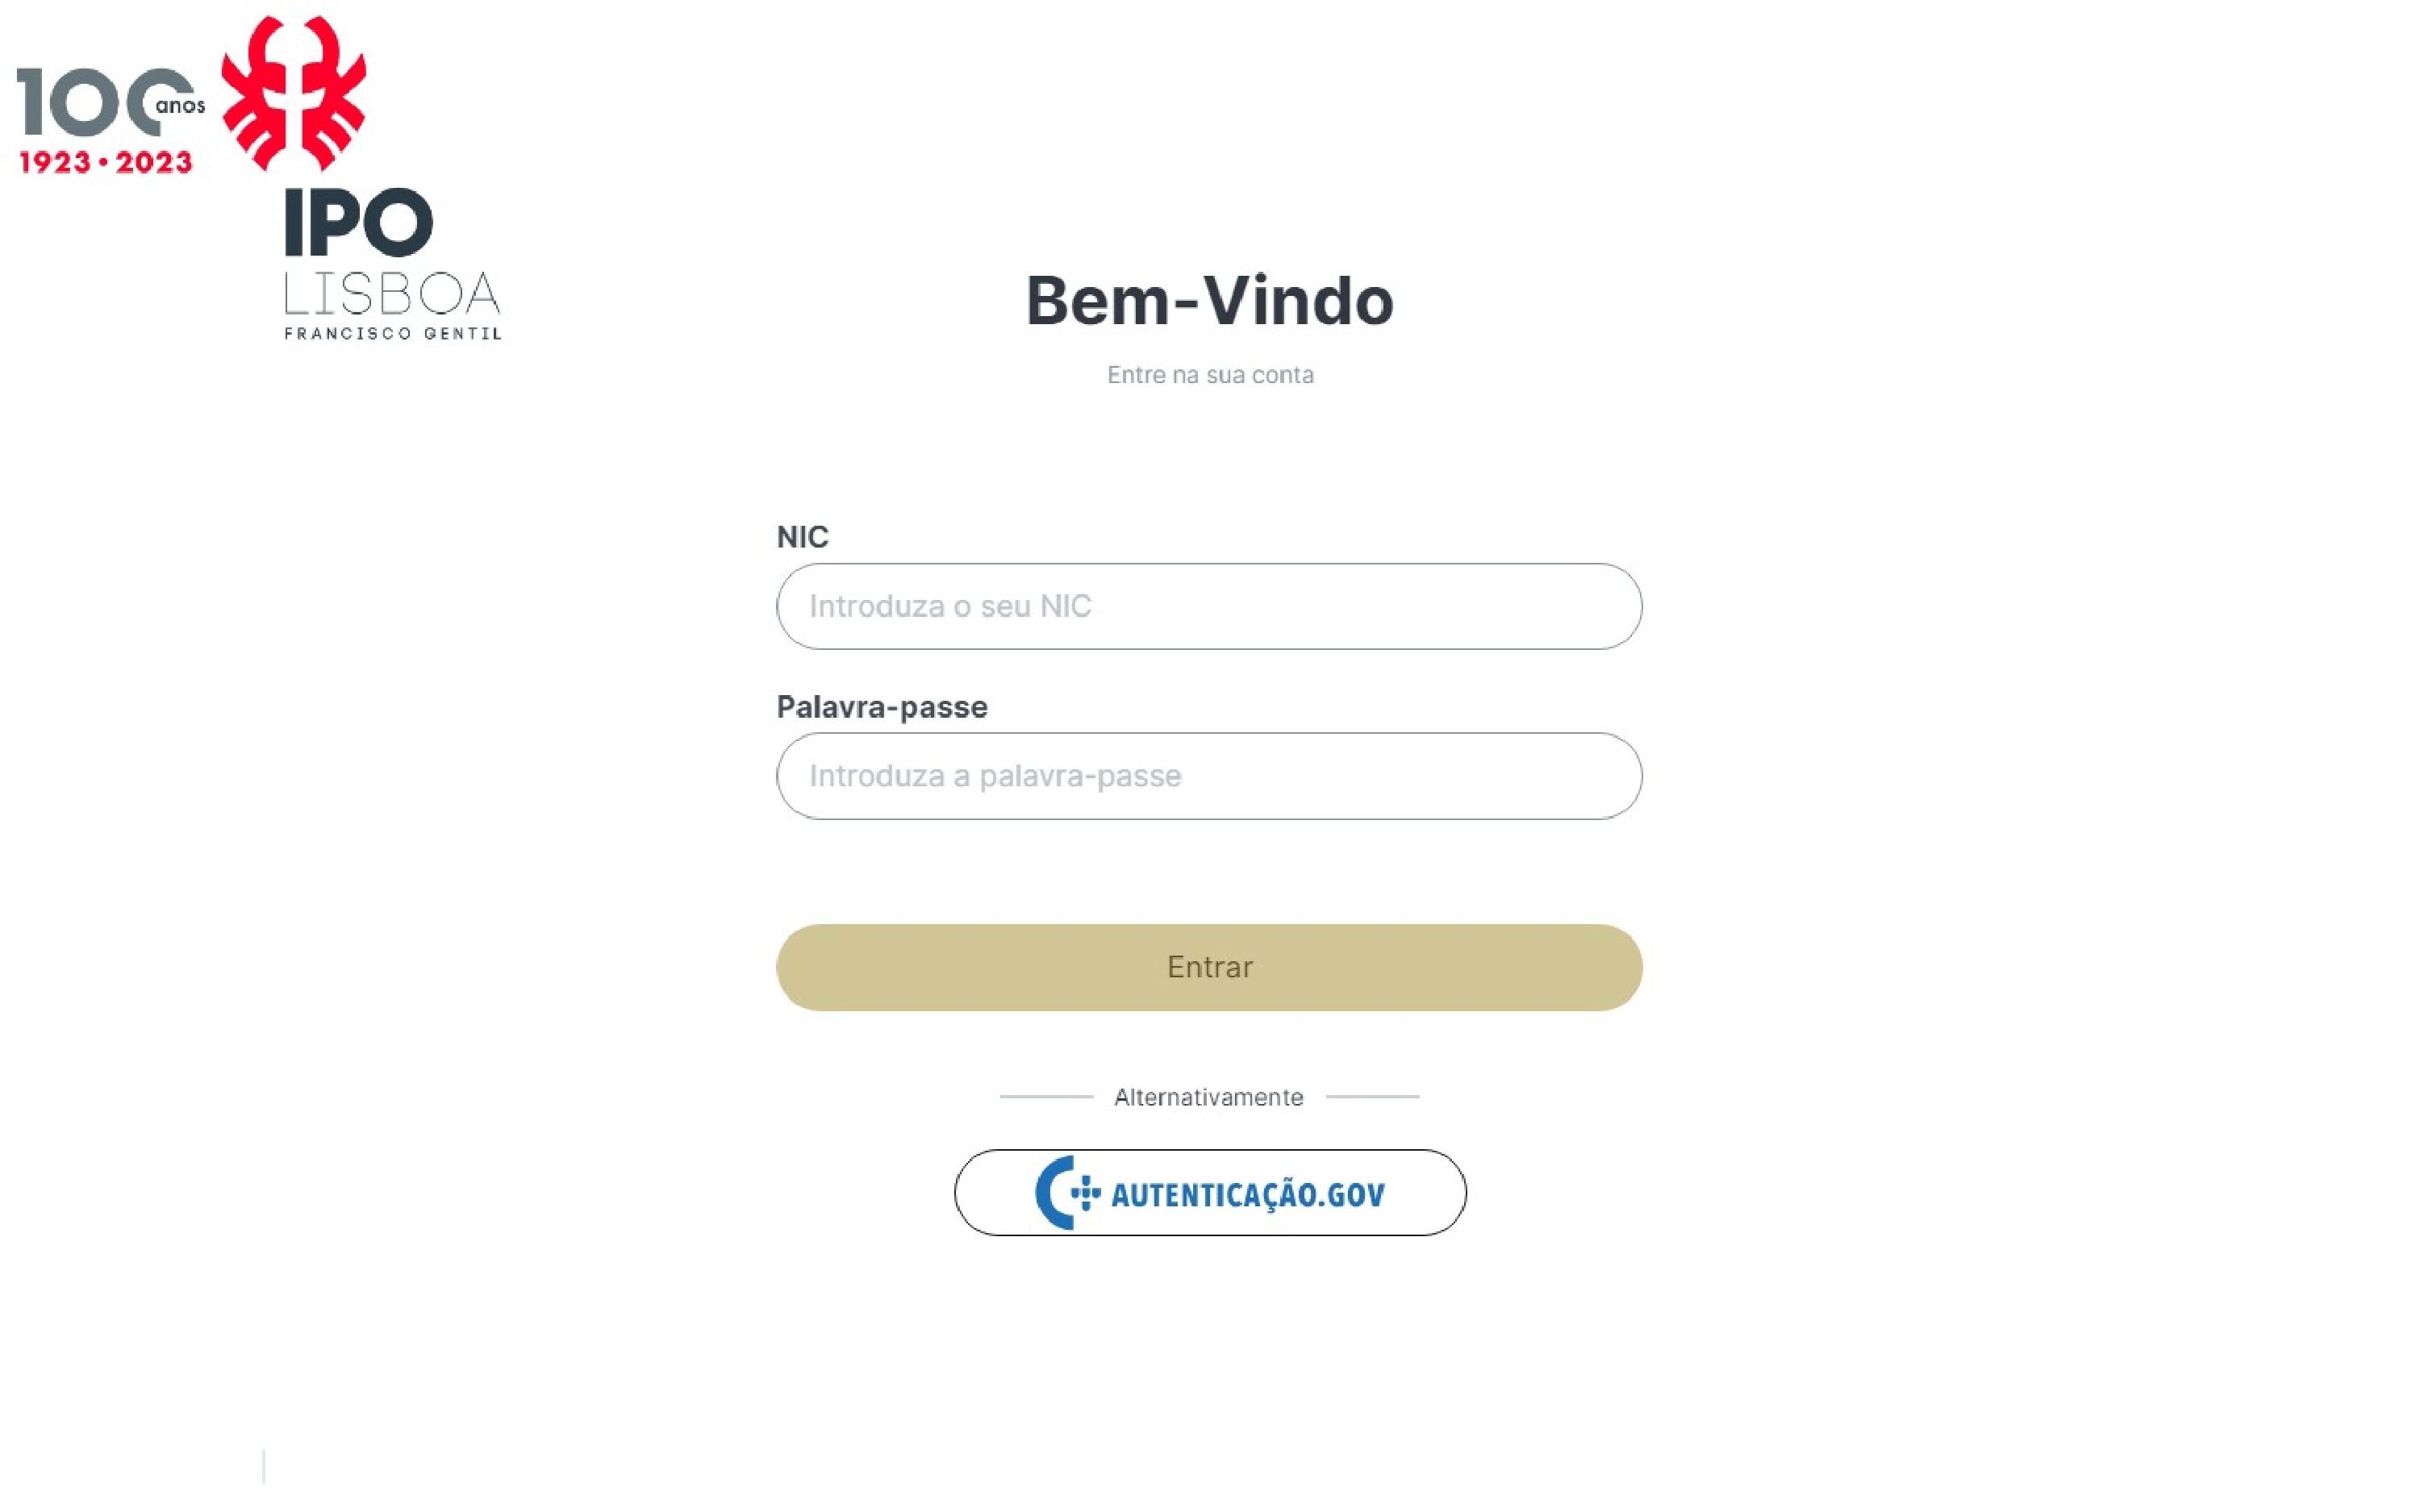
\includegraphics{./figures/Login.pdf}}
	\end{center}
	\caption{Login Page Mock.}\label{fig:login}
\end{figure}

\begin{figure}[H]
	\begin{center}
		\resizebox{160mm}{!}{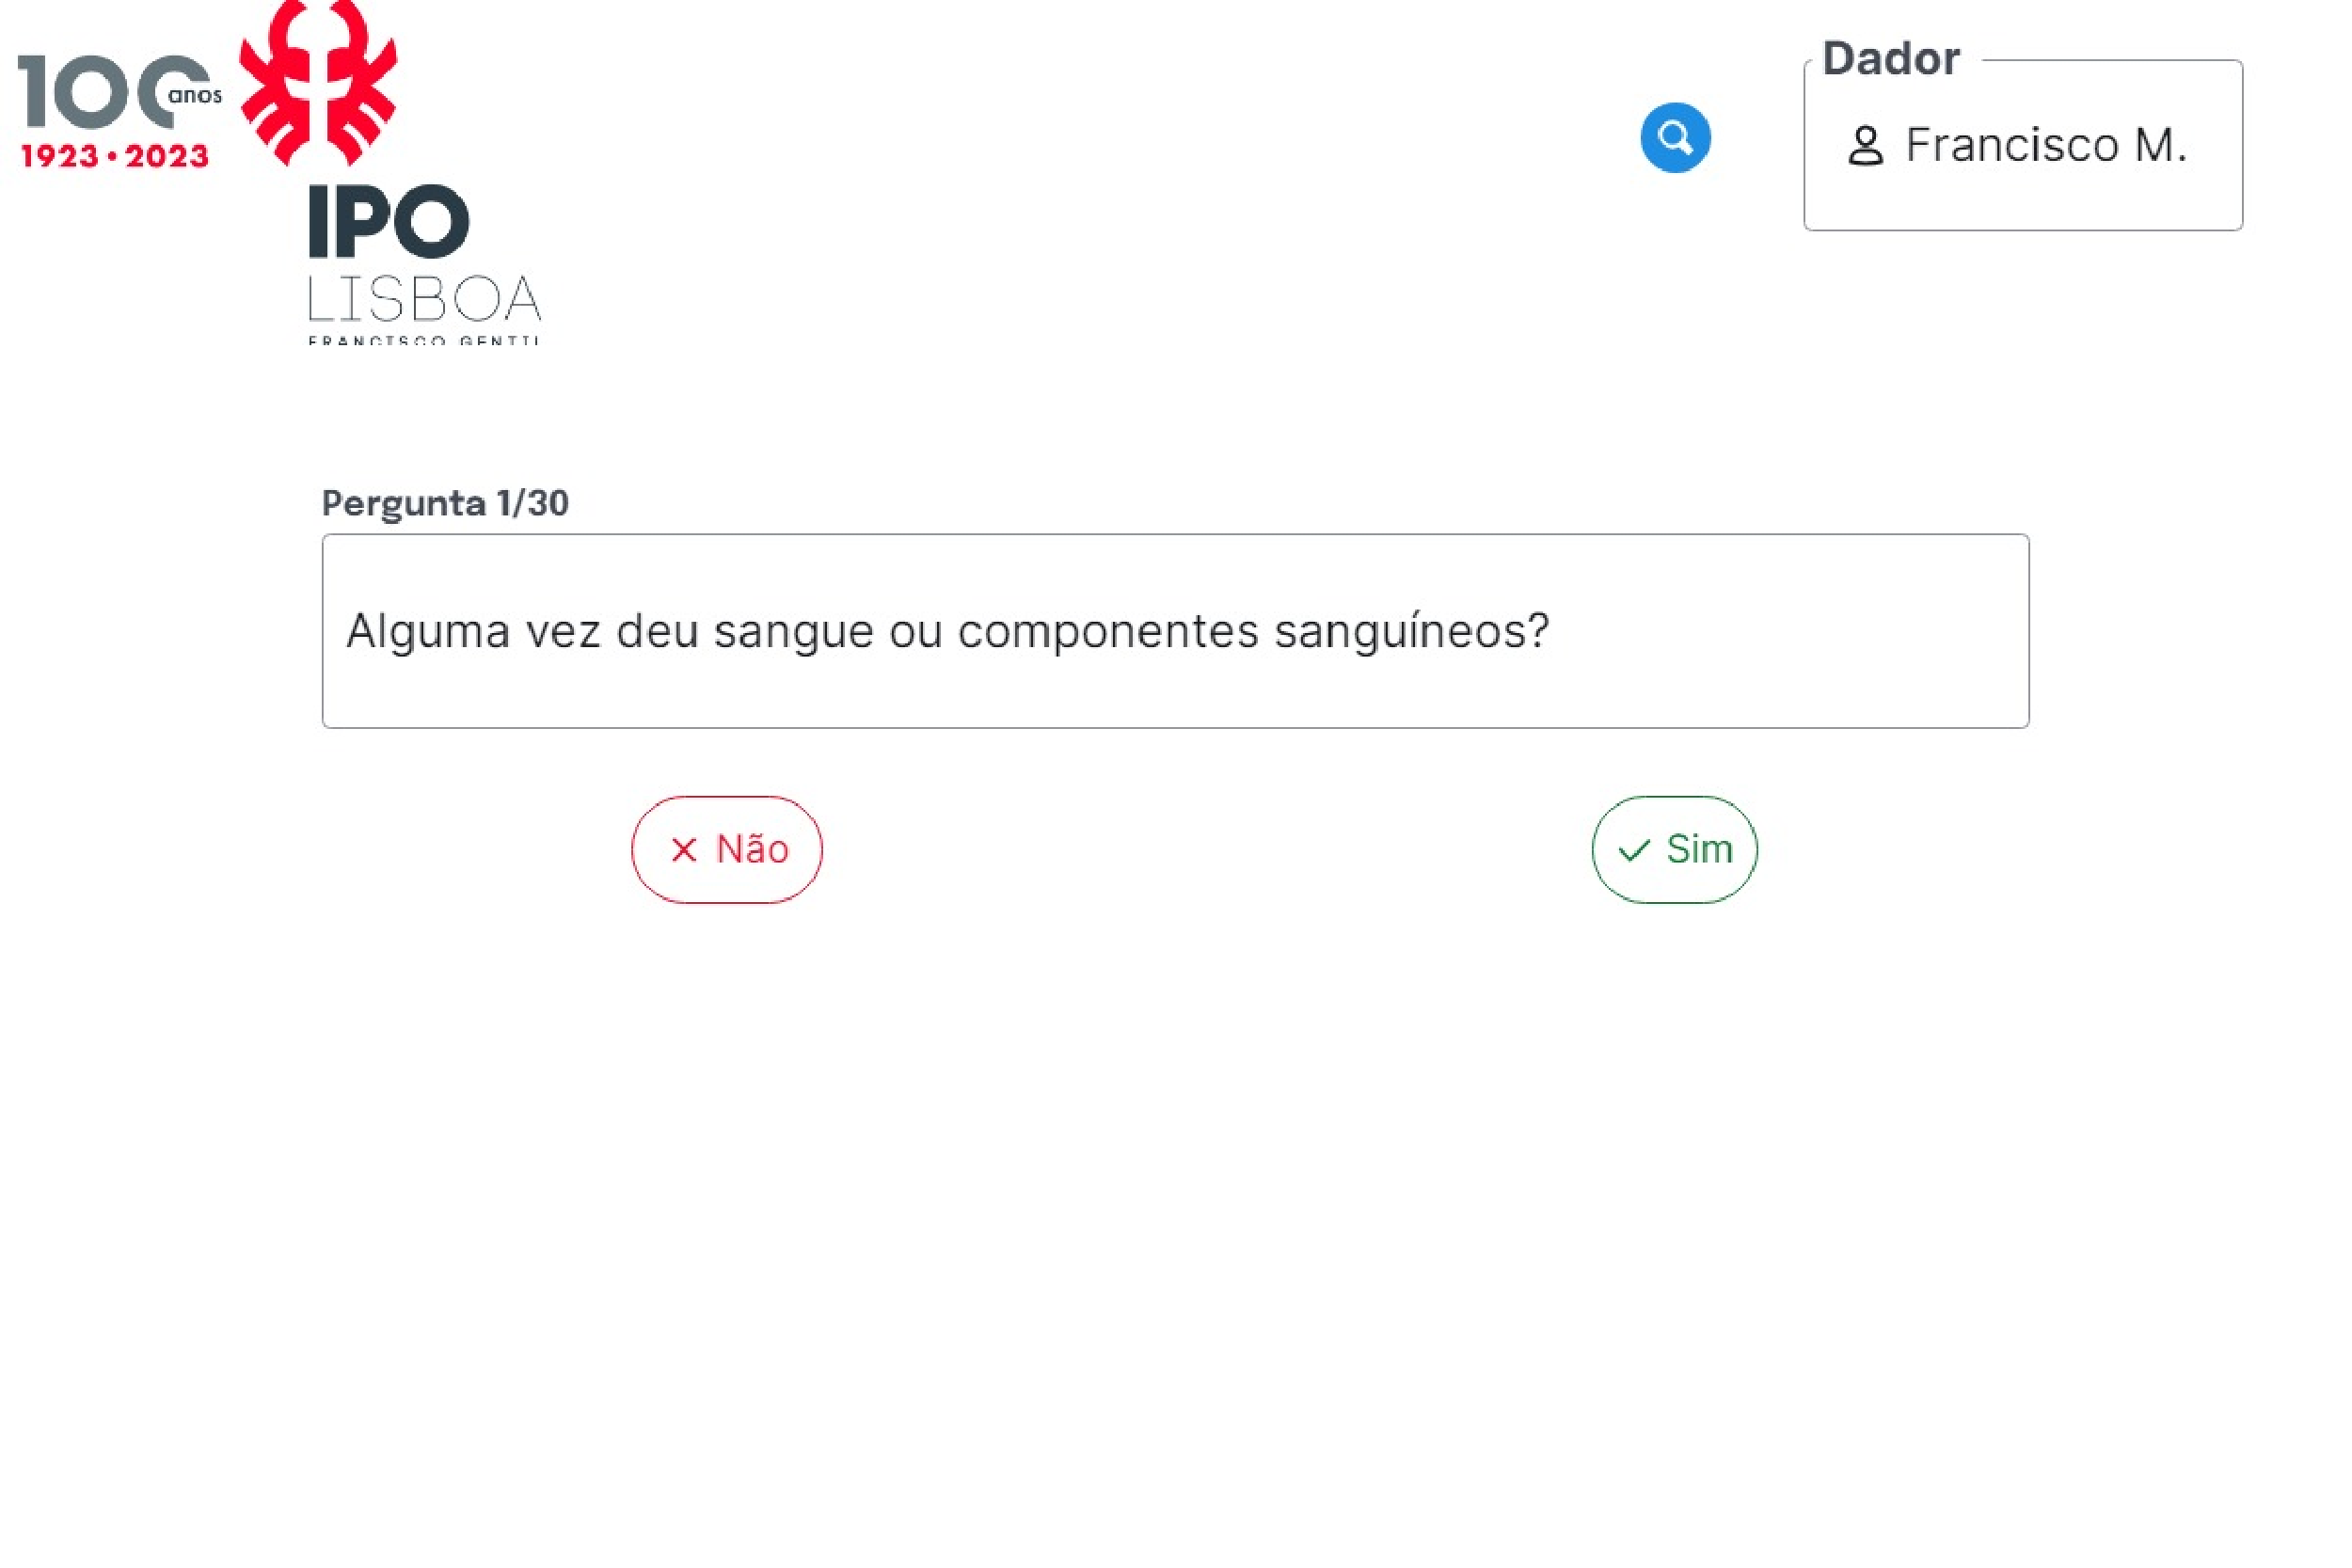
\includegraphics{./figures/Form.pdf}}
	\end{center}
	\caption{Form Page Mock.}\label{fig:form}
\end{figure}

\begin{figure}[H]
	\begin{center}
		\resizebox{160mm}{!}{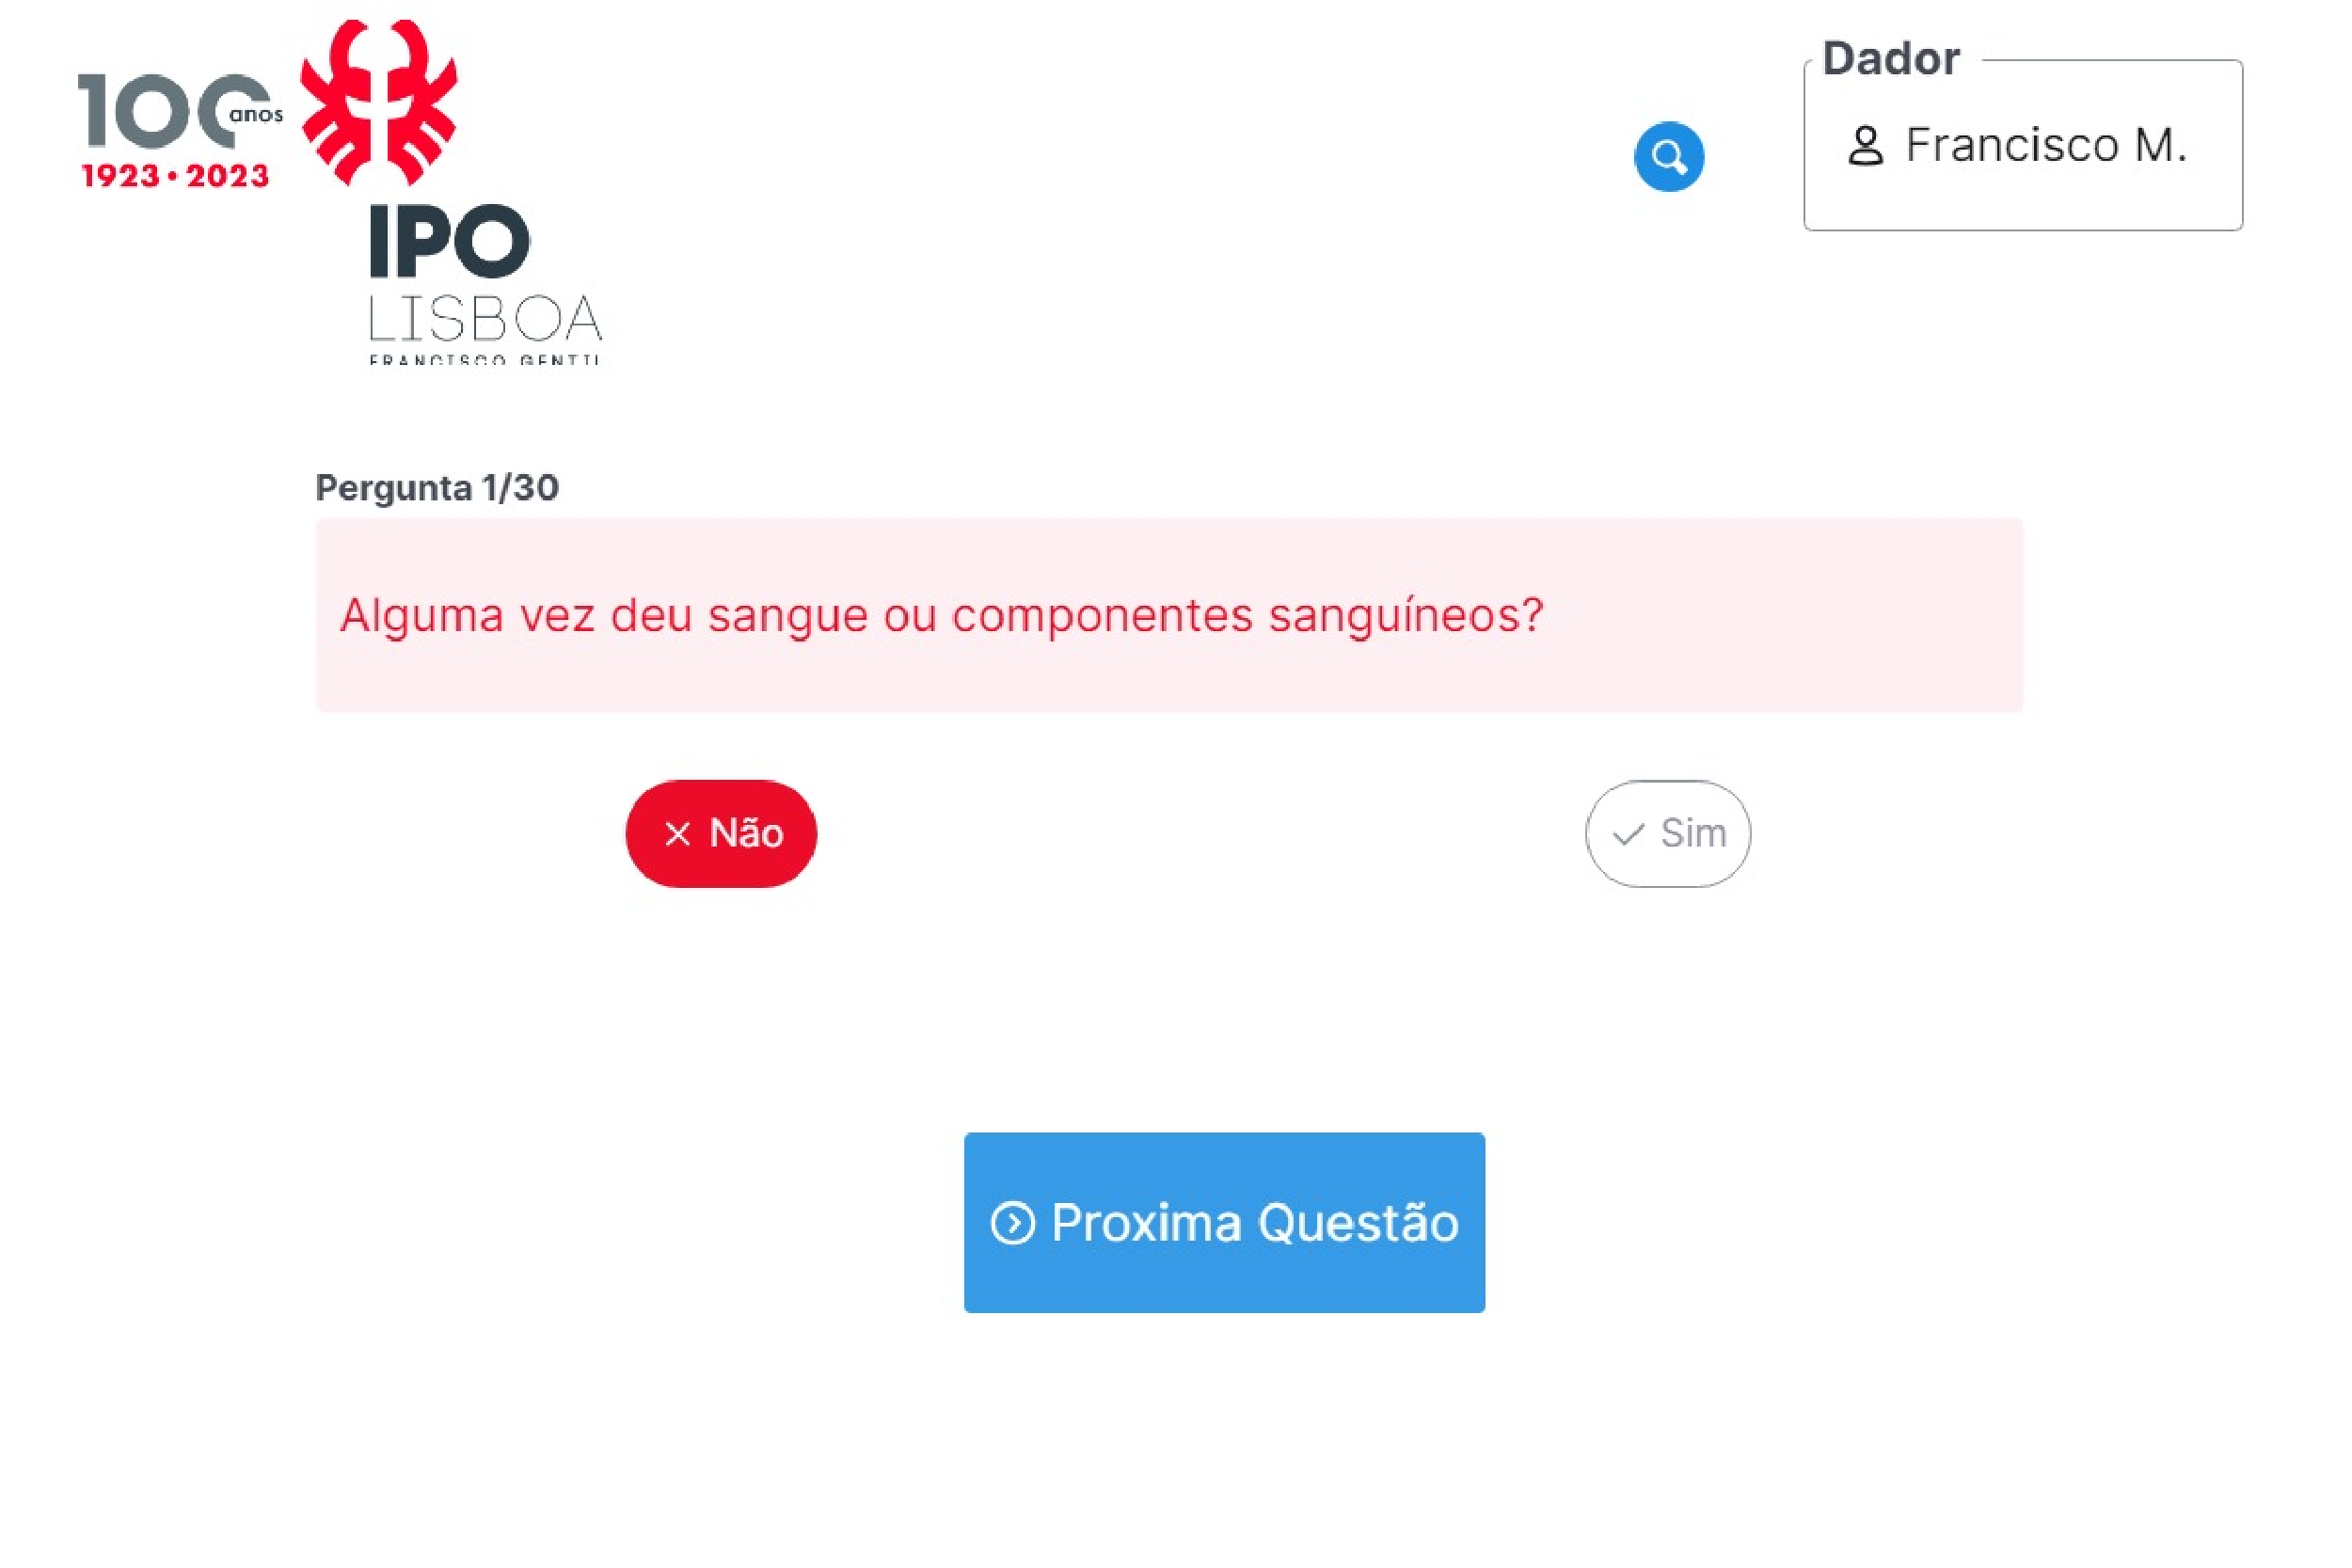
\includegraphics{./figures/Form_Answer_No.pdf}}
	\end{center}
	\caption{Form Page Negative Answer Mock.}\label{fig:form_no}
\end{figure}

\begin{figure}[H]
	\begin{center}
		\resizebox{160mm}{!}{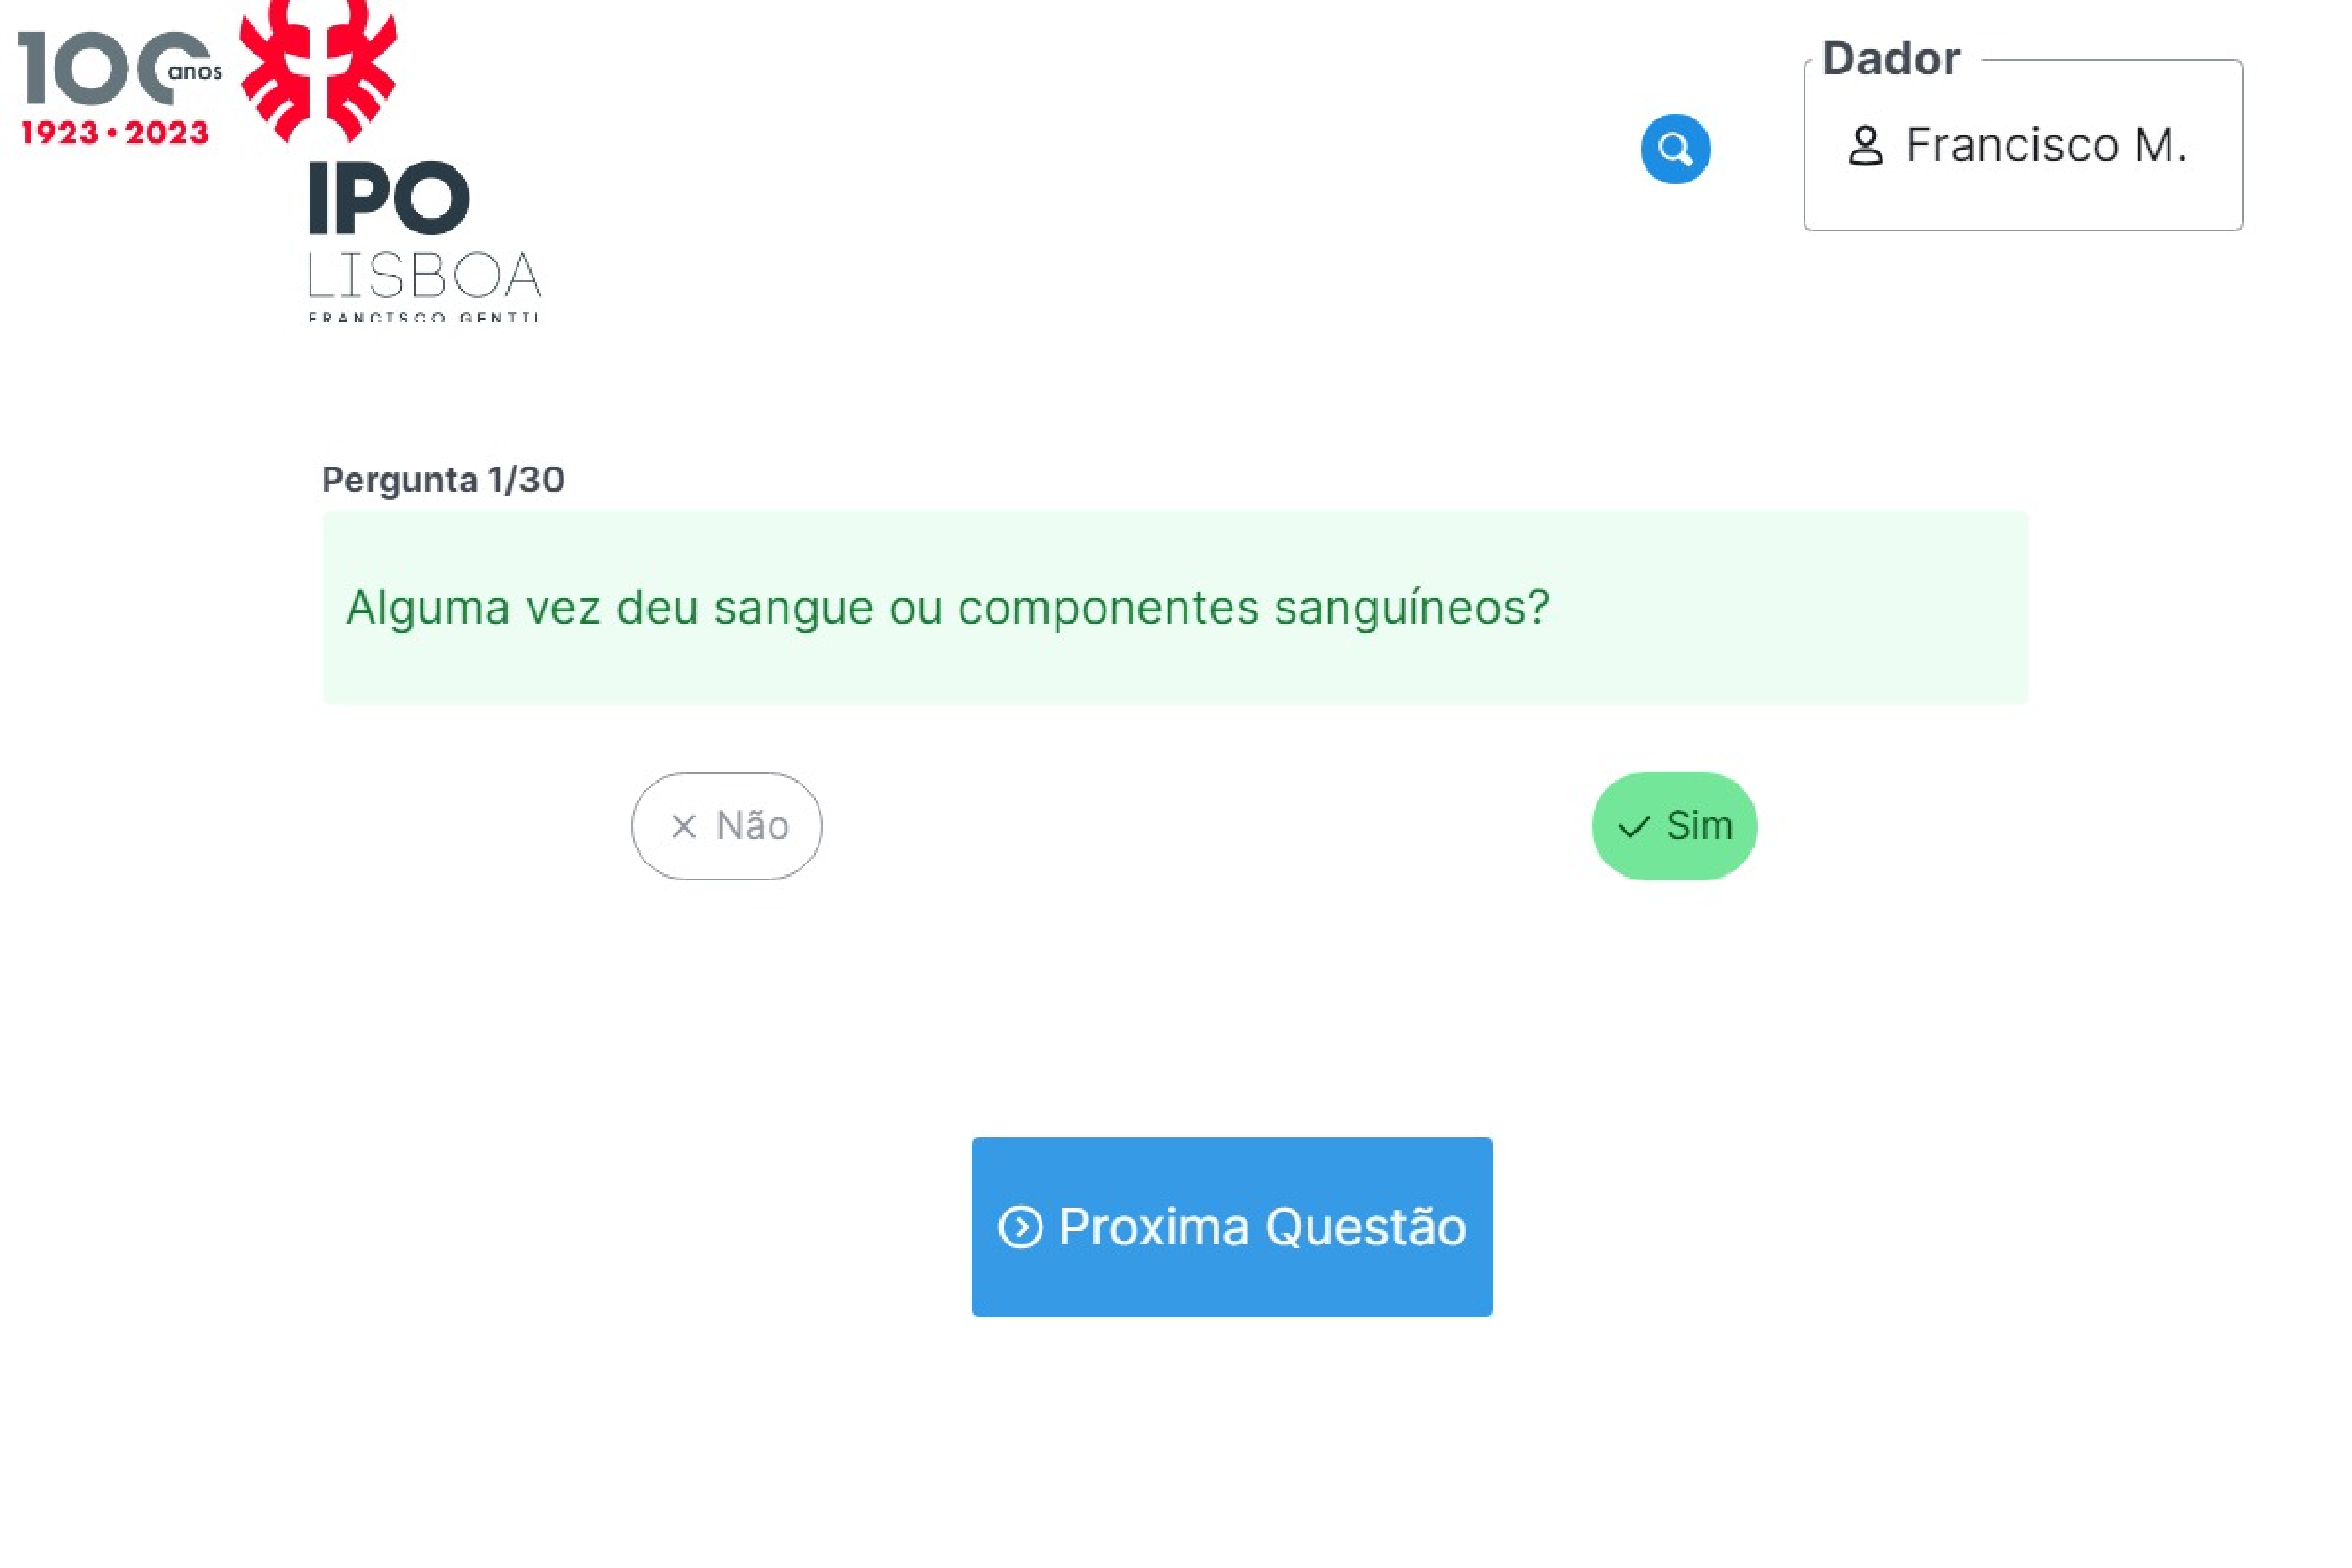
\includegraphics{./figures/Form_Answer_Yes.pdf}}
	\end{center}
	\caption{Form Page Positive Answer Mock.}\label{fig:form_yes}
\end{figure}

\begin{figure}[H]
	\begin{center}
		\resizebox{160mm}{!}{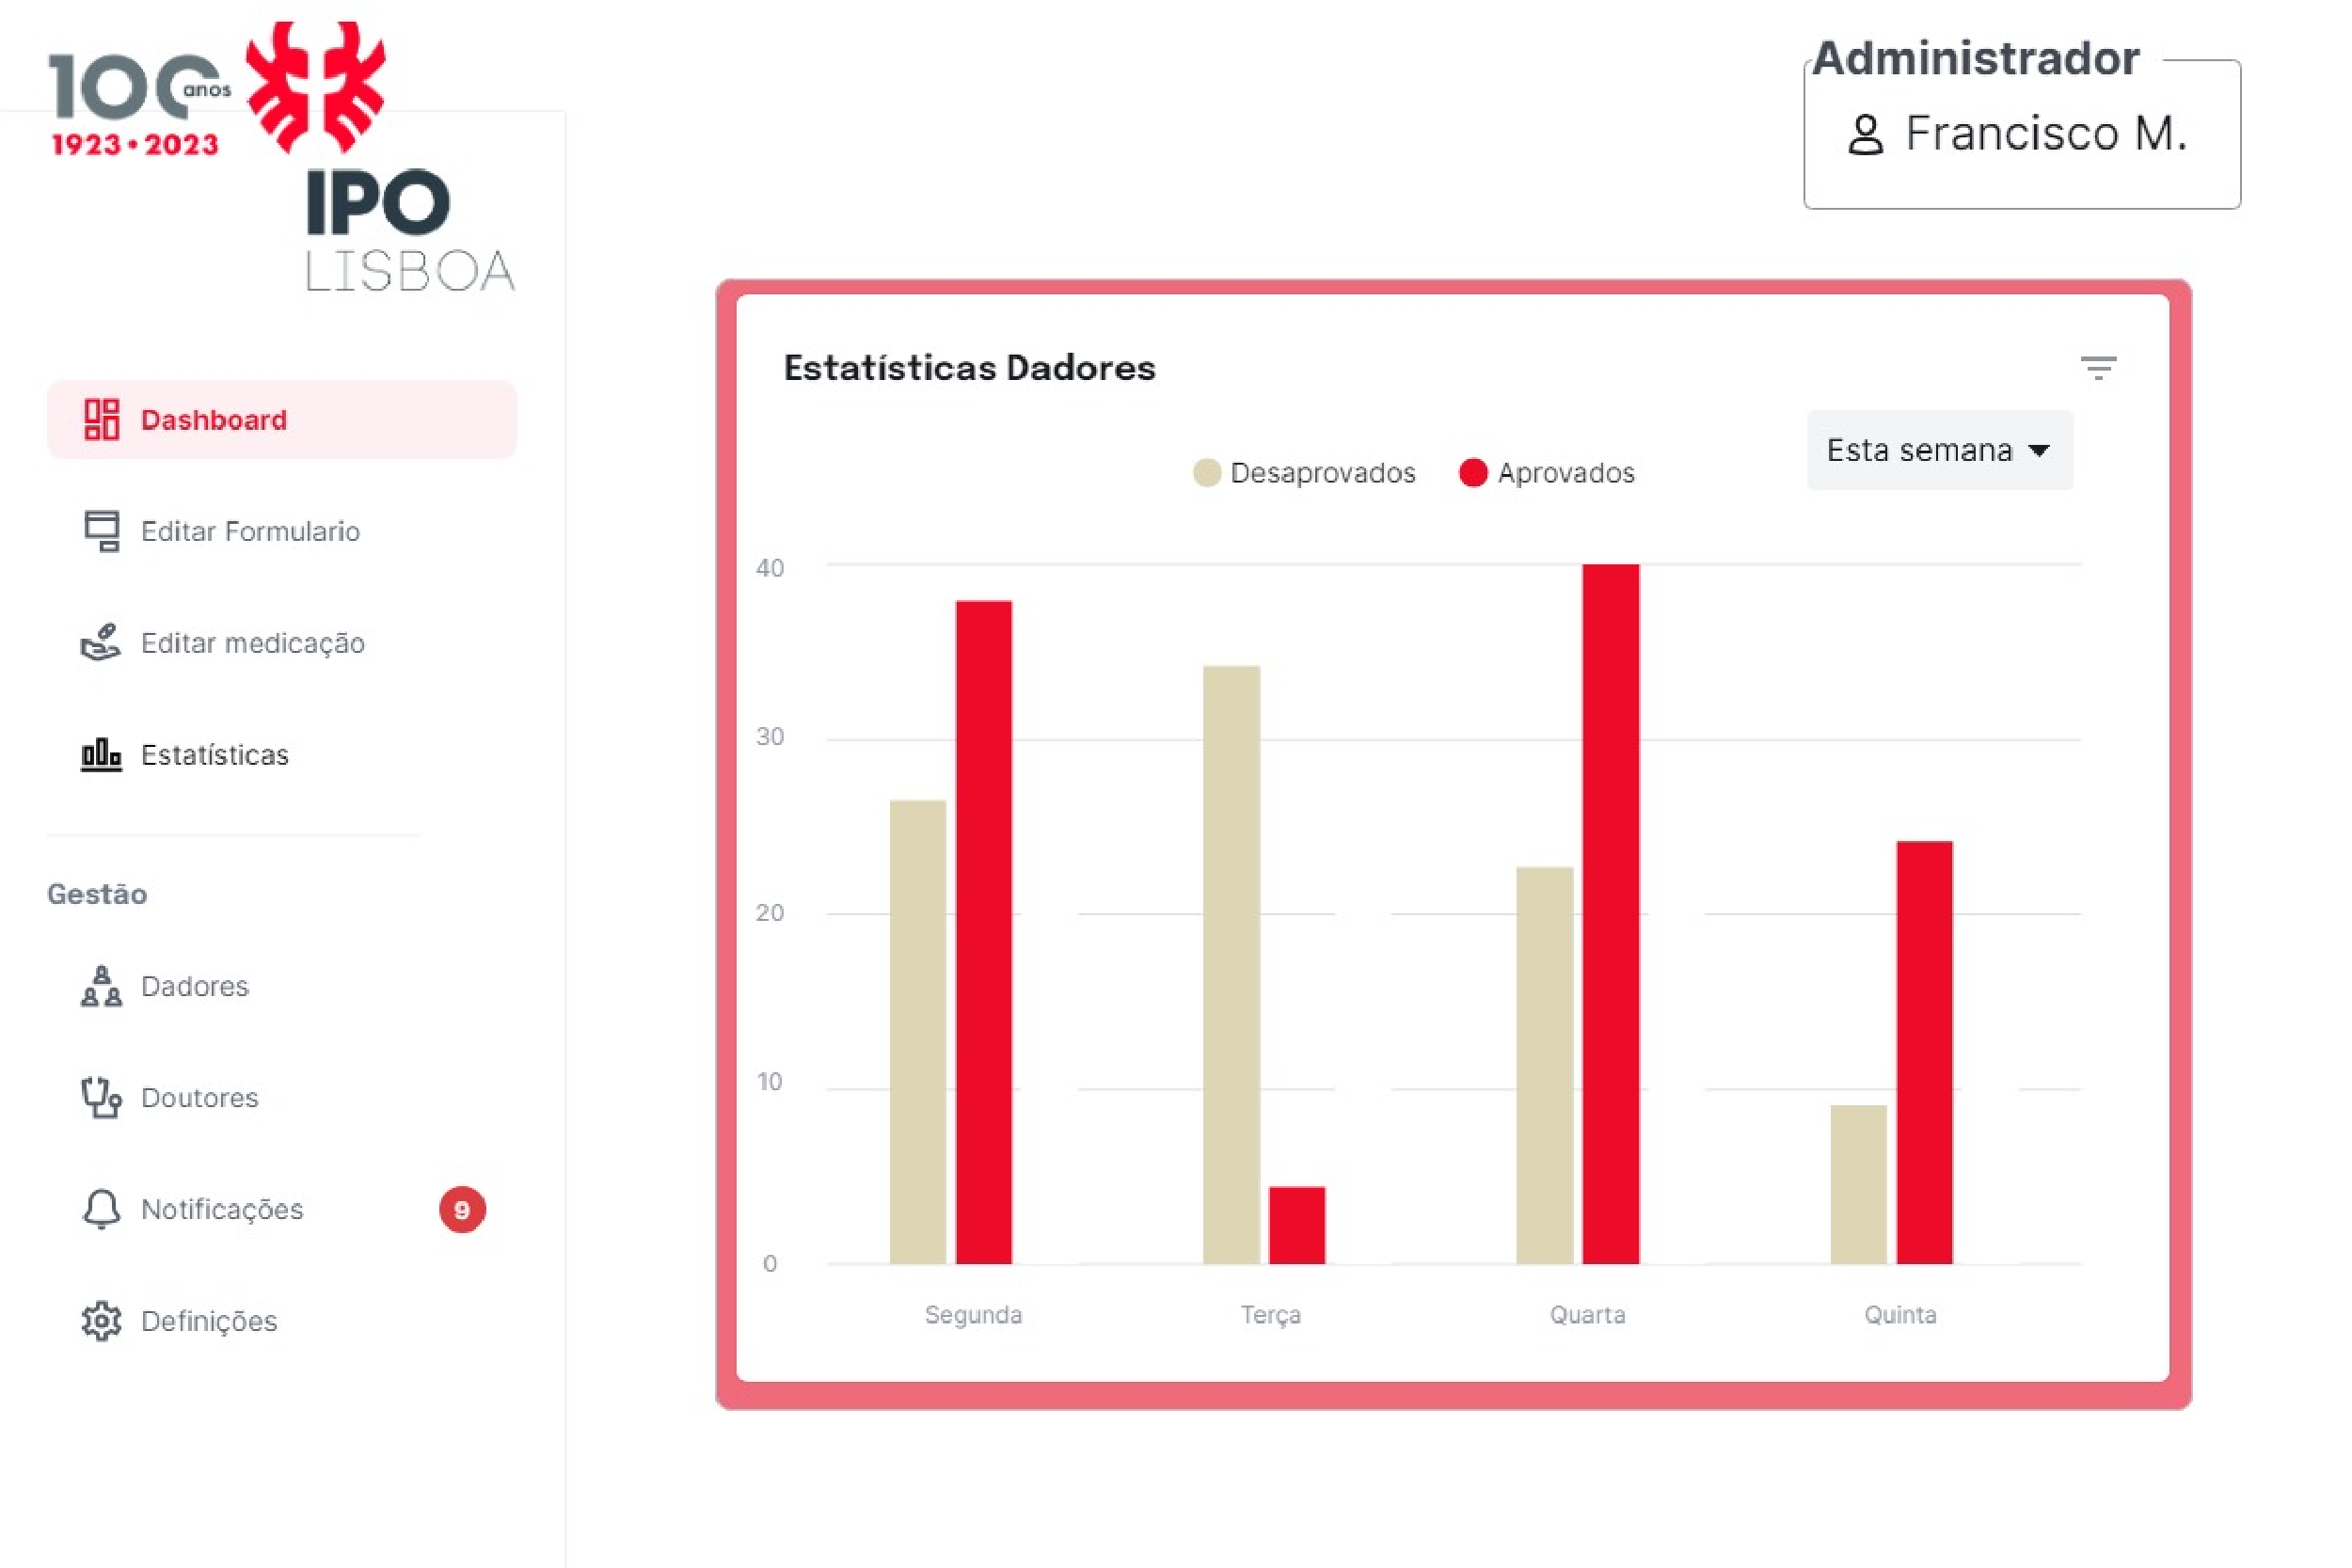
\includegraphics{./figures/Backoffice.pdf}}
	\end{center}
	\caption{Backoffice Page Mock.}\label{fig:backoffice}
\end{figure}




%\subsection{Form Services}
%
%The form service is responsible for managing the form resources.
%Figure ~\ref{fig:form_services} is a diagram that shows the architecture of the form services.
%
%\begin{figure}[htbp]
%	\begin{center}
%		\resizebox{150mm}{!}{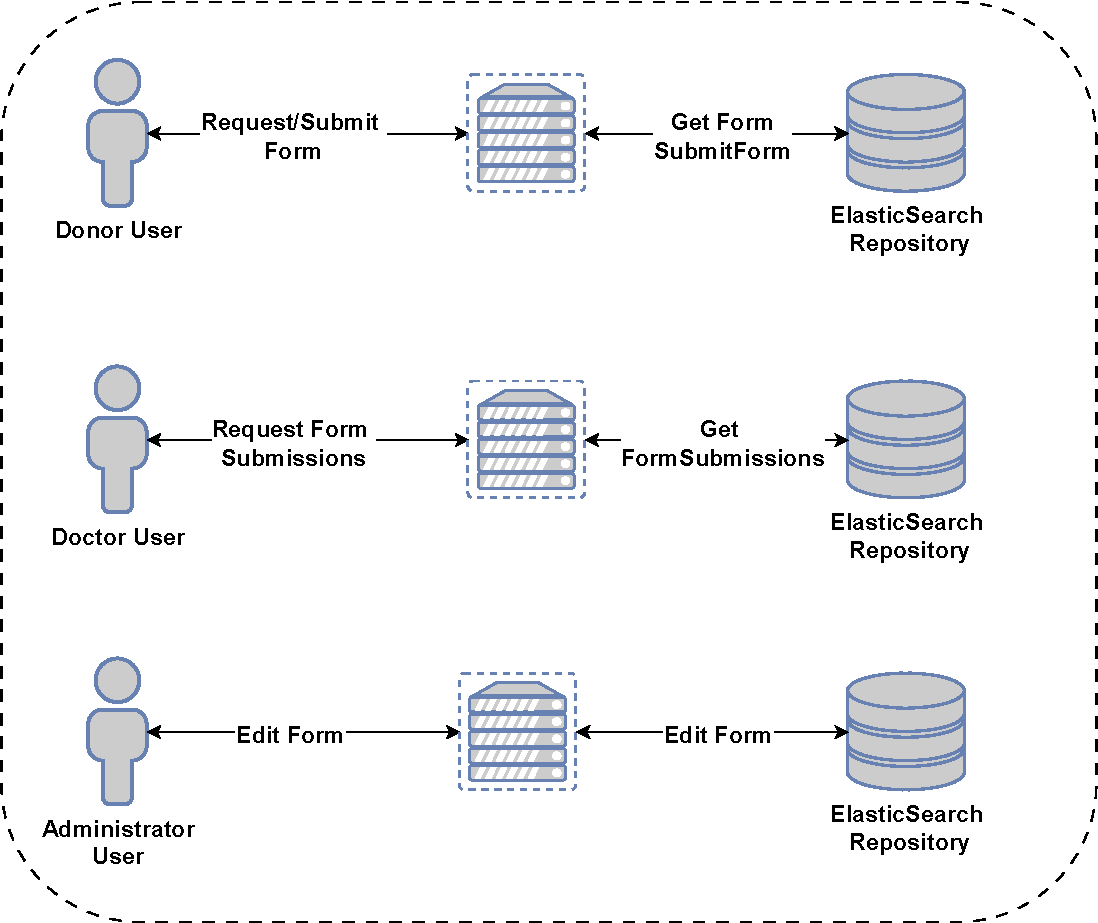
\includegraphics{./figures/formServices.pdf}}
%	\end{center}
%	\caption{Final Form Data Structure.}\label{fig:form_services}
%\end{figure}
